% Chapter 2

\chapter{Guidelines on Adjustments} % Main chapter title

\label{Chapter2} % For referencing the chapter elsewhere, use \ref{Chapter2} 

%----------------------------------------------------------------------------------------

% Define some commands to keep the formatting separated from the content 
% \newcommand{\keyword}[1]{\textbf{#1}}

%----------------------------------------------------------------------------------------
This chapter demonstrates how to make changes and DIY the thesis style when using this template. For each component of the thesis, we provide both 

\section{Title Page}
\textbf{Title Page} is designed to obviously bear the title of the thesis and the author's name. Users can add any degrees or professional qualifications that he/she holds as well as the author's name in the national script. Both the title and the author's name are highlighted in blod style. Given that there may also be an oral and/or written examination, and thus this template uses the following form of words:

\begin{quote}
A thesis submitted in partial fulfilment of the requirements for the degree of Doctor (or Master) of Philosophy at The University of Hong Kong.
\end{quote}

\noindent The title page is not numbered, or counted in the pagination of the front mater, or listed in the table of contents. The document for title page is quite simple, which can be found in the path \colorbox{gray!20}{Titlepage/titlepage.tex}.


\section{Dedication}
\label{chap2:sec2:dedication}
\textbf{Dedication} is a place to show your wish to dedicate the thesis to friends, family or loved ones. This template uses a single page example for dedication, as shown in \figref{fig:chap2:dedication_sample}. This page is not numbered, or counted in the pagination of the front matter, or listed in the table of contents.
\begin{figure}
    \centering
    
\includegraphics[width=.6\textwidth]{Dedication/dedication.pdf}
    \caption{An example dedication page.}
    \label{fig:chap2:dedication_sample}
\end{figure}


\section{Epigraph}
\label{chap2:sec3:epigraph}
\textbf{Epigraph} is a relevant quotation on the subject of the thesis, or some general guidelines or philosophical principles. Ordinarily, the author and source of the quotation should also be given. This page is not included in the template and users can add the epigraph page according to their willingness.


\section{Declarations}
\label{chap2:sec4:declarations}
\textbf{Declarations} page is a required item according to the official booklet. The contents of declaration are in terms of the official sample (\textit{Sample Page 6} on page 41 of the booklet) with some minor changes to specify the author's name and thesis title.


\section{Acknowledgements}
\label{chap2:sec5:acknowledgements}
\textbf{Acknowledgements} is the place where the author thanks mentors, labmates, colleagues, friends, family members and also the financial support from scholarships and research grants. Each page of the acknowledgements is numbered in lower case Roman numerals


\section{Table of Contents}
\label{chap2:sec6:table_of_contents}
\textbf{Table of Contents} in this template is simply headed ``Contents'' which lists all the parts of the thesis and the page on which they commence. Each of the chapters, sections and subsections are included in the list. The capitalization and wording of the titles listed in the table exactly agree with the corresponding ones appear in the body text. If users would like to include some optional pages in the Table of Contents, such as the Frontispiece page or Epigraph page, they can simply add a command \verb|\addchaptertocentry{\pagename}| at the corresponding page. For example, your can add the \textit{Abstract} item to the Table of Contents, by adding the command to the file \codestyle{Abstract/abstract.tex}, as shown in \figref{fig:chap2:example_add_command}.
\begin{figure}[!h]
    \centering
    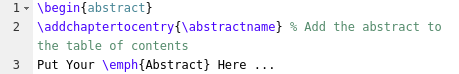
\includegraphics[width=.8\textwidth]{Figures/Chapter2/add_command_example.png}
    \caption{An example of how to add chapter to the Table of Contents.}\label{fig:chap2:example_add_command}
\end{figure}


\section{List of Tables, Figures and Algorithms, etc}
\label{chap2:sec7:list_of_tables_figures_and_algorithms_etc}
\begin{figure}[t]
    \centering
    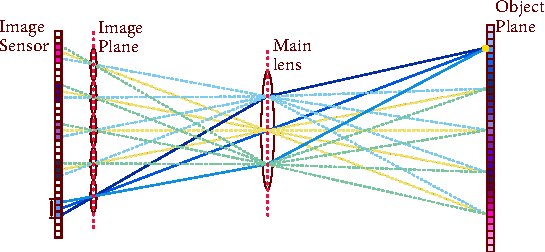
\includegraphics[width=0.6\textwidth]{Figures/Chapter2/photo_consistency.pdf}
    \caption{Light transformation model in a plenoptic camera. Within a plenoptic camera, a micro-lens array has been placed at the image plane, which further splits the incoming light rays from different directions and records them separately. Therefore, the multi-view information can be extracted from each light field image captured by a single shot.}
    \label{fig:photo_consistency}
\end{figure}

\begin{figure}[t]
    \centering
    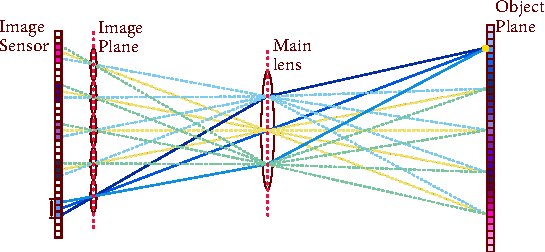
\includegraphics[width=0.6\textwidth]{Figures/Chapter2/photo_consistency.pdf}
    \caption[Light transformation model (focused on the plane).]{Light transformation model in a plenoptic camera. Within a plenoptic camera, a micro-lens array has been placed at the image plane, which further splits the incoming light rays from different directions and records them separately. Therefore, the multi-view information can be extracted from each light field image captured by a single shot.}
    \label{fig:photo_consistency_with_nickname}
\end{figure}
Following the Table of Contents, the template includes the lists of tables, figures and algorithms, abbreviations and symbols. The numbering, capitalisation and wording of the titles of every items listed agree exactly with the manner in which they appear in the body text. For the illustration with a long title, users can also provide a ``nickname'' of the illustration by enclosing the it in the square brackets. For example, \figref{fig:photo_consistency} and \figref{fig:photo_consistency_with_nickname} have the same image captions in the body text, but the wordings appear in the Table of Contents are different. \figref{fig:photo_consistency_with_nickname} uses the wordings in the square brackets as its caption, as shown at page \darkred{vii}.
